\documentclass[border=6pt]{standalone}
\usepackage{tikz}
\usetikzlibrary{arrows.meta,calc,positioning}
\begin{document}
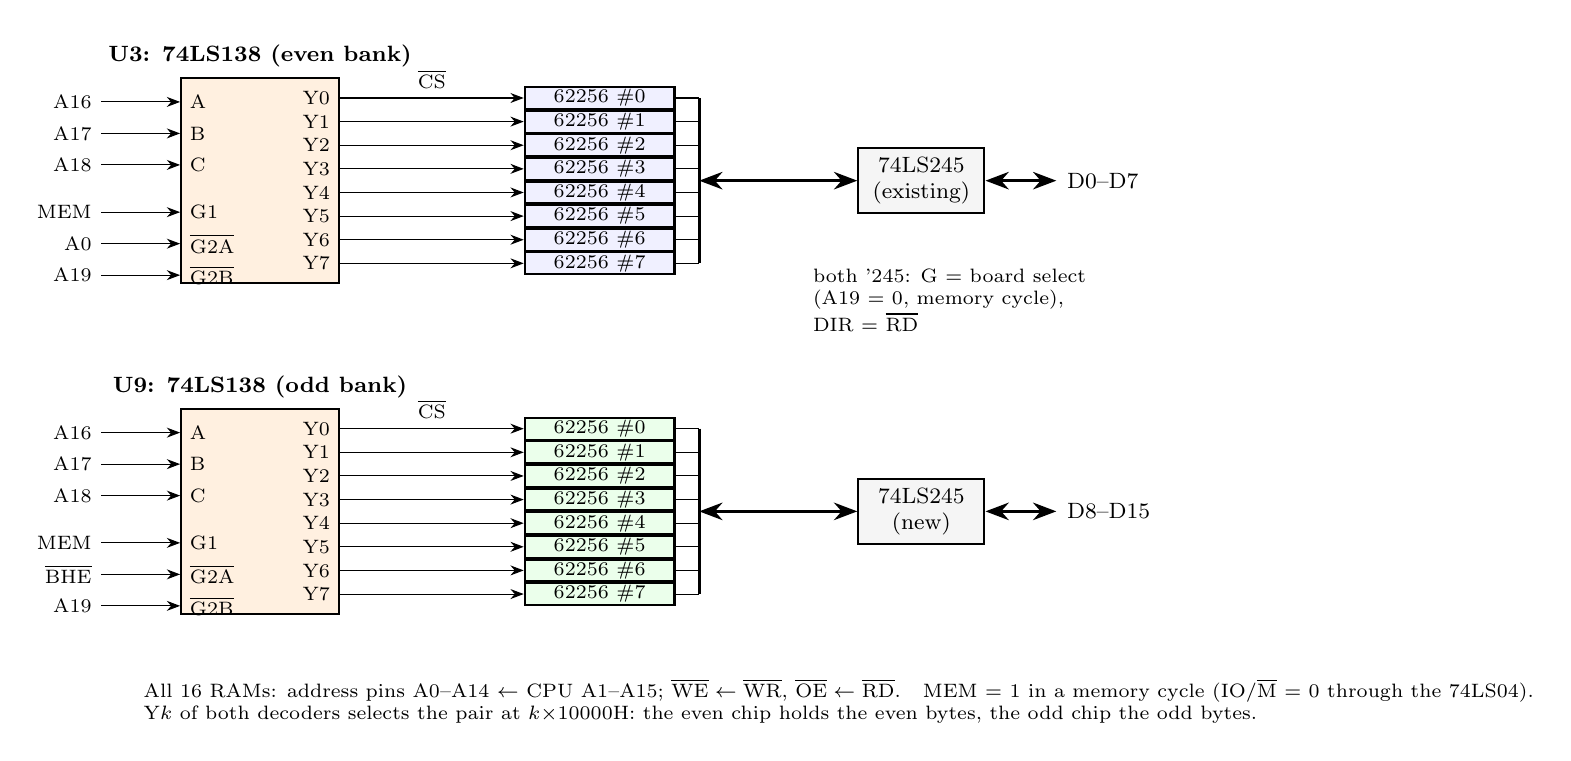
\begin{tikzpicture}[>=Stealth,font=\small,
 dec/.style={draw,thick,fill=orange!12,minimum width=2.0cm,minimum height=2.6cm},
 ram/.style={draw,thick,minimum width=1.9cm,minimum height=0.28cm,font=\tiny,inner sep=0pt},
 tr/.style={draw,thick,fill=gray!8,minimum width=1.6cm,minimum height=0.8cm,font=\footnotesize,align=center}]
% decoders
\foreach \d/\y/\col/\gtwoa/\name in {U3/0/blue!6/A0/even,U9/-4.2/green!8/$\overline{\mathrm{BHE}}$/odd} {
  \node[dec] (\d) at (0,\y) {};
  \node[font=\footnotesize\bfseries,anchor=south] at (\d.north) {\d: 74LS138 (\name\ bank)};
  \foreach \p/\dy in {A/1.0,B/0.6,C/0.2,G1/-0.4,$\overline{\mathrm{G2A}}$/-0.8,$\overline{\mathrm{G2B}}$/-1.2} \node[font=\scriptsize,anchor=west] at ($(\d.west)+(0,\dy)$) {\p};
  \foreach \s/\dy in {A16/1.0,A17/0.6,A18/0.2,MEM/-0.4,\gtwoa/-0.8,A19/-1.2} \draw[<-] ($(\d.west)+(0,\dy)$) -- ++(-1.0,0) node[left,font=\scriptsize]{\s};
  \foreach \k in {0,...,7} {
    \node[font=\scriptsize,anchor=east] at ($(\d.east)+(0,1.05-0.3*\k)$) {Y\k};
    \node[ram,fill=\col] (r\d\k) at ($(\d.east)+(3.3,1.05-0.3*\k)$) {};
  }
  \draw[->] ($(\d.east)+(0,1.05)$) -- (r\d0.west) node[pos=0.5,above,font=\scriptsize]{$\overline{\mathrm{CS}}$};
  \foreach \k in {1,...,7} \draw[->] ($(\d.east)+(0,1.05-0.3*\k)$) -- (r\d\k.west);
  \foreach \k in {0,...,7} \node[font=\scriptsize] at (r\d\k) {62256 \#\k};
}
\node[font=\scriptsize,align=left,anchor=north west] at (-1.4,1.95) {};
% data paths
\node[tr] (t1) at (8.4,0.0) {74LS245\\(existing)};
\node[tr] (t2) at (8.4,-4.2) {74LS245\\(new)};
\foreach \d/\t in {U3/t1,U9/t2} {
  \foreach \k in {0,...,7} \draw (r\d\k.east) -- ++(0.3,0);
  \draw[very thick] ($(r\d0.east)+(0.3,0)$) -- ($(r\d7.east)+(0.3,0)$);
  \draw[<->,very thick] ($(r\d3.east)!0.5!(r\d4.east)+(0.3,0)$) -- (\t.west |- {$(r\d3.east)!0.5!(r\d4.east)$}) ;
}
\draw[<->,very thick] (t1.east) -- ++(0.9,0) node[right,font=\footnotesize]{D0--D7};
\draw[<->,very thick] (t2.east) -- ++(0.9,0) node[right,font=\footnotesize]{D8--D15};
\node[font=\scriptsize,align=left,anchor=north west] at (6.9,-1.0) {both '245: G = board select\\(A19 = 0, memory cycle),\\DIR = $\overline{\mathrm{RD}}$};
% common
\node[font=\scriptsize,align=left,anchor=north west] at (-1.6,-6.2) {All 16 RAMs: address pins A0--A14 $\leftarrow$ CPU A1--A15; $\overline{\mathrm{WE}} \leftarrow \overline{\mathrm{WR}}$, $\overline{\mathrm{OE}} \leftarrow \overline{\mathrm{RD}}$.\quad MEM = 1 in a memory cycle (IO/$\overline{\mathrm{M}}$ = 0 through the 74LS04).\\
Y$k$ of both decoders selects the pair at $k\times$10000H: the even chip holds the even bytes, the odd chip the odd bytes.};
\end{tikzpicture}
\end{document}
